\documentclass{article}
\usepackage{amsmath}
\usepackage{amssymb}
\usepackage{graphicx}
\usepackage{hyperref}
\usepackage[version=4]{mhchem}

\title{Problem 8}
\date{}

\begin{document}
\maketitle

\section*{Problem}
Triangle \(A B C . A B=n A C . A P\) is the angle bisector of \(\angle A . B P \perp A P\). \(A P\) and \(B C\) meet at \(Q\). Show that \(P Q: Q A=(n-1): 2\).\\
\centering
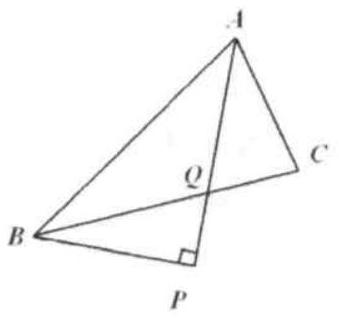
\includegraphics[width=\textwidth]{images/127(4).jpg}

\section*{Solution}
Solution not available.

\end{document}
